\subthesischapter{Manipulación de los datos}
SQLite ha sido favorecido por los desarrolladores móviles y recomendado por la documentación oficial de Android. Aún Unity no ha brindado soporte oficial para crear bases de datos. Sin embargo, se ha ideado una manera de utilizar las ventajas de SQLite para nuestra aplicación.

La idea utilizada fue agrupar los métodos y variables comunes en una clase. Luego extender la clase usando herencia para crear implementaciones reales. Fue creada una clase de alto nivel \underline{DataBaseModel}  que se puede extender a otras clases, con el fin de acceder a las operaciones básicas de cualquier base de datos. Llamamos a estas operaciones básicas CURD: Crear, Actualizar, Leer y Borrar, (ver Figura \ref{fig: diagram-db}).

\begin{figure}[ht]
    \centering
    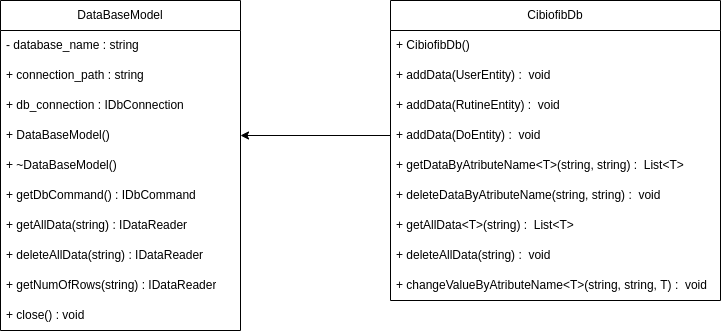
\includegraphics[scale=0.6]{images/diagram-db.png}
    \caption{Diagrama de clases}
    \label{fig: diagram-db}
\end{figure}

Para gestionar la información almacenada en la base de datos del sistema, se ha implementado un conjunto de funciones en C\# utilizando la biblioteca System.Data.SQLite. Estas funciones permiten realizar las operaciones CURD sobre las tablas USER, RUTINE y DO.

\begin{itemize}
    \item \underline{Conexión con la base de datos:} Para establecer la conexión con la base de datos, se utiliza la función getDbCommand() que devuelve un objeto de tipo IDbCommand. Este objeto se utiliza para ejecutar las instrucciones SQL en la base de datos. Se asegura que la conexión esté establecida correctamente antes de realizar cualquier operación de manipulación de datos.
    
    \item \underline{Inserción en la base de datos:} Para insertar nuevos registros en las tablas USER, RUTINE o DO, se han implementado las funciones addData(UserEntity user), addData(RutineEntity rutine) y addData(DoEntity \_do) respectivamente. Estas funciones generan y ejecutan instrucciones SQL del tipo INSERT INTO para agregar nuevos registros a las tablas. Los datos son obtenidos de objetos de las clases UserEntity, RutineEntity y DoEntity definidas en Models.cs.

    \item \underline{Obtención de datos:} Para obtener datos de la base de datos, se han implementado las funciones getDataByAtributeName<T>(string atribute, string name) y getAllData<T>(string table\_name). La primera función permite obtener datos específicos de una tabla según un atributo y un valor dado. La segunda función recupera todos los registros de una tabla específica. Ambas funciones devuelven los datos en forma de listas de objetos del tipo especificado por el tipo genérico T.

    \item \underline{Eliminación de registros:} Para eliminar los datos de la base de datos, se han implementado las funciones deleteDataByAtributeName(string atribute, string name) y deleteAllData(string table\_name). La primera función permite eliminar datos específicos de una tabla según un atributo y un valor dado. La segunda función elimina todos los registros de una tabla específica.

    \item \underline{Edicion de atributos en la base de datos:} Para la edición de los datos en la base de datos, se implementó la función changeValueByAtributeName<T>(string atribute, string name, T value), que permite editar los datos de un atributo a partir de un valor genérico dado.
\end{itemize}